% =====================================================================
%  OpenHydroQual -- presentation for Dewberry
%  Arash Massoudieh, EnviroInformatics LLC / The Catholic University of America
%
%  Build:   latexmk -pdf main.tex        (or: pdflatex main.tex  x2)
%
%  FIGURES: every image is a \figslot. If the file is not in figures/,
%  a red-labelled placeholder is drawn instead and the item is listed on
%  the "Figure checklist" slide at the end. Drop the file into figures/
%  under the name printed on the placeholder and it is picked up on the
%  next build -- no edits needed.
% =====================================================================
\documentclass[aspectratio=169, 10pt]{beamer}
\usetheme{metropolis}
\metroset{progressbar=frametitle, sectionpage=progressbar, numbering=fraction}

% ---------------------------------------------------------------
% OpenHydroQual -- Dewberry presentation : preamble & figure slots
% ---------------------------------------------------------------
\usepackage[T1]{fontenc}
\usepackage[utf8]{inputenc}
\usepackage{graphicx}
\usepackage{booktabs}
\usepackage{tikz}
\usepackage{xcolor}
\usepackage{listings}
\usepackage{amsmath}
\usetikzlibrary{positioning,arrows.meta,shapes.geometric,fit,backgrounds,calc}

\graphicspath{{figures/}}

% ---- brand colours -------------------------------------------------
\definecolor{ohqblue}{HTML}{1F5C8B}
\definecolor{ohqteal}{HTML}{2A9D8F}
\definecolor{ohqsand}{HTML}{E9C46A}
\definecolor{ohqrust}{HTML}{E76F51}
\definecolor{ohqgrey}{HTML}{6B7280}
\definecolor{phfill}{HTML}{F1F2F4}
\definecolor{phline}{HTML}{A8B0BA}

\setbeamercolor{alerted text}{fg=ohqrust}
\setbeamercolor{progress bar}{fg=ohqteal}
\setbeamercolor{title separator}{fg=ohqteal}

% ---- code listing style --------------------------------------------
\lstdefinestyle{ohqshell}{
  basicstyle=\ttfamily\scriptsize,
  keywordstyle=\color{ohqteal}\bfseries,
  commentstyle=\color{ohqgrey}\itshape,
  stringstyle=\color{ohqblue},
  showstringspaces=false,
  breaklines=true,
  frame=single,
  rulecolor=\color{phline},
  backgroundcolor=\color{phfill},
  columns=fullflexible,
  keepspaces=true,
}
\lstset{style=ohqshell}

% ====================================================================
%  FIGURE SLOT MACHINERY
%
%  \figslot{ID}{filename}{width}{caption/what to capture}
%
%  If figures/<filename> exists it is included at <width>.
%  If not, a dashed placeholder box is drawn showing the ID and the
%  description of what still needs to be captured, and the ID is added
%  to the checklist printed by \printfigurechecklist.
%
%  ==> To fill a slot: drop the file into figures/ under the exact
%      name shown on the placeholder. Nothing else to edit.
% ====================================================================
\makeatletter
% height cap applied to a FILLED \figslot; raise it on a frame whose image is
% the point of the slide (\setlength{\figslotmaxht}{0.82\textheight}).
\newlength{\figslotmaxht}
\setlength{\figslotmaxht}{0.66\textheight}
\newcommand{\ohq@missinglist}{}
\newcounter{ohq@nmissing}
\newcounter{ohq@nfilled}

\newcommand{\figslot}[4]{%
  \IfFileExists{figures/#2}{%
    \stepcounter{ohq@nfilled}%
    \begin{center}\includegraphics[width=#3,height=\figslotmaxht,keepaspectratio]{#2}\end{center}%
  }{%
    \stepcounter{ohq@nmissing}%
    \g@addto@macro\ohq@missinglist{\item \textbf{#1}: \texttt{\detokenize{#2}}\\[-2pt] {\footnotesize\color{ohqgrey} #4}}%
    \begin{center}%
    \begin{tikzpicture}
      \node[draw=phline, dashed, thick, fill=phfill, rounded corners=3pt,
            minimum width=#3, minimum height=\dimexpr#3*46/100\relax,
            align=center, inner sep=8pt, text width=\dimexpr#3-30pt\relax]
        (box) {%
          {\color{ohqrust}\bfseries\large #1}\\[4pt]
          {\color{ohqgrey}\ttfamily\scriptsize \detokenize{figures/#2}}\\[7pt]
          {\color{black!70}\small #4}%
        };
      \node[anchor=north east, font=\tiny\bfseries, color=white,
            fill=ohqrust, rounded corners=2pt, inner sep=3pt]
        at ([shift={(-4pt,-4pt)}]box.north east) {NEEDED};
    \end{tikzpicture}%
    \end{center}%
  }%
}

% compact variant for side-by-side use inside columns
\newcommand{\figslotmini}[4]{%
  \IfFileExists{figures/#2}{%
    \stepcounter{ohq@nfilled}%
    \includegraphics[width=#3,height=0.58\textheight,keepaspectratio]{#2}%
  }{%
    \stepcounter{ohq@nmissing}%
    \g@addto@macro\ohq@missinglist{\item \textbf{#1}: \texttt{\detokenize{#2}}\\[-2pt] {\footnotesize\color{ohqgrey} #4}}%
    \begin{tikzpicture}
      \node[draw=phline, dashed, fill=phfill, rounded corners=3pt,
            minimum width=#3, minimum height=\dimexpr#3*58/100\relax,
            align=center, inner sep=5pt, text width=\dimexpr#3-18pt\relax]
        {{\color{ohqrust}\bfseries\footnotesize #1}\\[3pt]
         {\color{black!70}\tiny #4}};
    \end{tikzpicture}%
  }%
}

\newcommand{\printfigurechecklist}{%
  \ifnum\value{ohq@nmissing}=0
    \begin{center}{\Large\color{ohqteal}\bfseries All figure slots are filled.}\end{center}
  \else
    {\footnotesize
     \begin{itemize}\setlength{\itemsep}{2pt}
       \ohq@missinglist
     \end{itemize}}
  \fi
}
\newcommand{\figurestats}{%
  \arabic{ohq@nmissing} outstanding%
}
\makeatother

% ---- small helpers --------------------------------------------------
\newcommand{\ohq}{\textsc{OpenHydroQual}}
\newcommand{\ohtwin}{\textsc{OpenHydroTwin}}
\newcommand{\keyfact}[1]{{\color{ohqblue}\bfseries #1}}

% ---- tighter typography so dense frames fit 16:9 --------------------
\setbeamerfont{itemize/enumerate body}{size=\footnotesize}
\setbeamerfont{itemize/enumerate subbody}{size=\scriptsize}
\setbeamerfont{itemize/enumerate subsubbody}{size=\scriptsize}
\setbeamerfont{frametitle}{size=\large}
\setlength{\leftmargini}{1.2em}
\setlength{\leftmarginii}{1.0em}
\addtolength{\parskip}{-0.25\baselineskip}
\setbeamertemplate{itemize item}{\color{ohqteal}\scriptsize$\blacktriangleright$}
\setbeamertemplate{itemize subitem}{\color{ohqgrey}\scriptsize$\triangleright$}

% ---- height-capped image helpers ------------------------------------
% \fitimg[width]{file}   -- never taller than 0.66\textheight
\newcommand{\fitimg}[2][\textwidth]{%
  \includegraphics[width=#1,height=0.66\textheight,keepaspectratio]{#2}}
% \fitimgs[width]{file}  -- shorter cap, for frames with text underneath
\newcommand{\fitimgs}[2][\textwidth]{%
  \includegraphics[width=#1,height=0.55\textheight,keepaspectratio]{#2}}
\setbeamerfont{section in toc}{size=\small}
\setbeamerfont{title}{size=\Large}
\setbeamerfont{subtitle}{size=\small}
\setbeamerfont{institute}{size=\scriptsize}
\setbeamerfont{date}{size=\scriptsize}

% \gridimg{file} -- for multi-image montage rows (height-capped per row)
\newcommand{\gridimg}[1]{%
  \includegraphics[width=\columnwidth,height=0.26\textheight,keepaspectratio]{#1}}

% ---- template montage (see make_icon_grid.py / icongrid.tex) --------
\newlength{\iconsize}
\setlength{\iconsize}{0.92cm}
\newlength{\iconrowgap}
\setlength{\iconrowgap}{0.10em}
\newlength{\iconlabelht}
\setlength{\iconlabelht}{0.72cm}

% ---- JSON listing style (real excerpts from resources/) -------------
\lstdefinelanguage{ohqjson}{
  morestring=[b]",
  morecomment=[l]{//},
  sensitive=true,
}
\lstdefinestyle{ohqjsonstyle}{
  language=ohqjson,
  basicstyle=\ttfamily\tiny,
  stringstyle=\color{ohqblue},
  commentstyle=\color{ohqgrey}\itshape,
  showstringspaces=false,
  breaklines=true,
  frame=single,
  rulecolor=\color{phline},
  backgroundcolor=\color{phfill},
  columns=fullflexible,
  keepspaces=true,
  aboveskip=2pt, belowskip=2pt,
  moredelim=[is][\color{ohqrust}\bfseries]{@@}{@@},
}


\title{OpenHydroQual}
\subtitle{An open, component-based platform for integrated water systems modeling}
% (subtitle kept short deliberately -- metropolis title page has little vertical room)
\author{Arash Massoudieh}
\institute{EnviroInformatics, LLC \quad\textbar\quad The Catholic University of America}
\date{Presentation to Dewberry \quad\textbar\quad \today}
% \titlegraphic{...} omitted -- metropolis' title page has no room for it;
% the logo appears on the closing slide instead.

\begin{document}

\maketitle

\begin{frame}{Roadmap}
  \setbeamertemplate{section in toc}[sections numbered]
  \begin{columns}[T,onlytextwidth]
    \begin{column}{0.48\textwidth}
      \tableofcontents[hideallsubsections, sections={1-4}]
    \end{column}
    \begin{column}{0.48\textwidth}
      \tableofcontents[hideallsubsections, sections={5-8}]
    \end{column}
  \end{columns}
\end{frame}

% =====================================================================
\section{What OpenHydroQual Is}
% =====================================================================

\begin{frame}{One engine, many water problems}
  \ohq{} is an \alert{open-source, component-based} platform for building and
  optimizing models of water systems, not a fixed-purpose model with a fixed
  set of processes.

  \vspace{0.4em}
  \begin{columns}[T,onlytextwidth]
    \begin{column}{0.48\textwidth}
      \textbf{Routinely used for}
      \begin{itemize}\setlength\itemsep{1pt}
        \item Rainfall--runoff and catchment hydrology
        \item Stormwater control measures / green infrastructure
        \item Sewer and pipe networks, pumps, tanks
        \item Open-channel flow, culverts, reservoirs
        \item Saturated and unsaturated subsurface flow
        \item Water quality, reactive transport, ASM
        \item Integrated urban water management
      \end{itemize}
    \end{column}
    \begin{column}{0.48\textwidth}
      \textbf{What makes it different}
      \begin{itemize}\setlength\itemsep{1pt}
        \item Every process component is a \alert{JSON plugin}, extensible
              without touching C++
        \item Symbolic equations and rules are part of the model file, and
              every input carries its own unit, SI or US customary
        \item Calibration and Bayesian uncertainty are \alert{built in}, not bolted on
        \item Same model file runs in the GUI, on a cluster, or inside a
              real-time digital twin
      \end{itemize}
    \end{column}
  \end{columns}
\end{frame}

\begin{frame}{The whole application}
  \setlength{\figslotmaxht}{0.86\textheight}
  \figslot{S1}{S1_main_window.png}{\textwidth}{%
    Screenshot: full \ohq{} main window with a visually rich model open,
    ideally a sewershed or water network with many blocks and links, property
    panel and item navigator both visible. This is the anchor image of the talk.}
\end{frame}

% =====================================================================
\section{How Models Are Built}
% =====================================================================

\begin{frame}{Blocks, links, sources, constituents}
  \figslot{N1}{N1_block_link_concept.pdf}{0.78\textwidth}{%
    New graphic: generic conceptual diagram with two blocks joined by a link,
    an external source feeding one of them, a constituent being transported,
    with the governing mass-balance ODE written underneath. The foundational
    ``how it works'' picture. (I can draw this in TikZ.)}

  \vspace{-0.3em}
  {\footnotesize A model is a network. Each \textbf{block} holds state
  (water volume, mass, energy, cost); each \textbf{link} carries a flux between
  blocks; \textbf{sources} inject external forcing; \textbf{constituents} ride
  along with their own reaction network.}
\end{frame}

\begin{frame}{The framework in one picture}
  \centering
  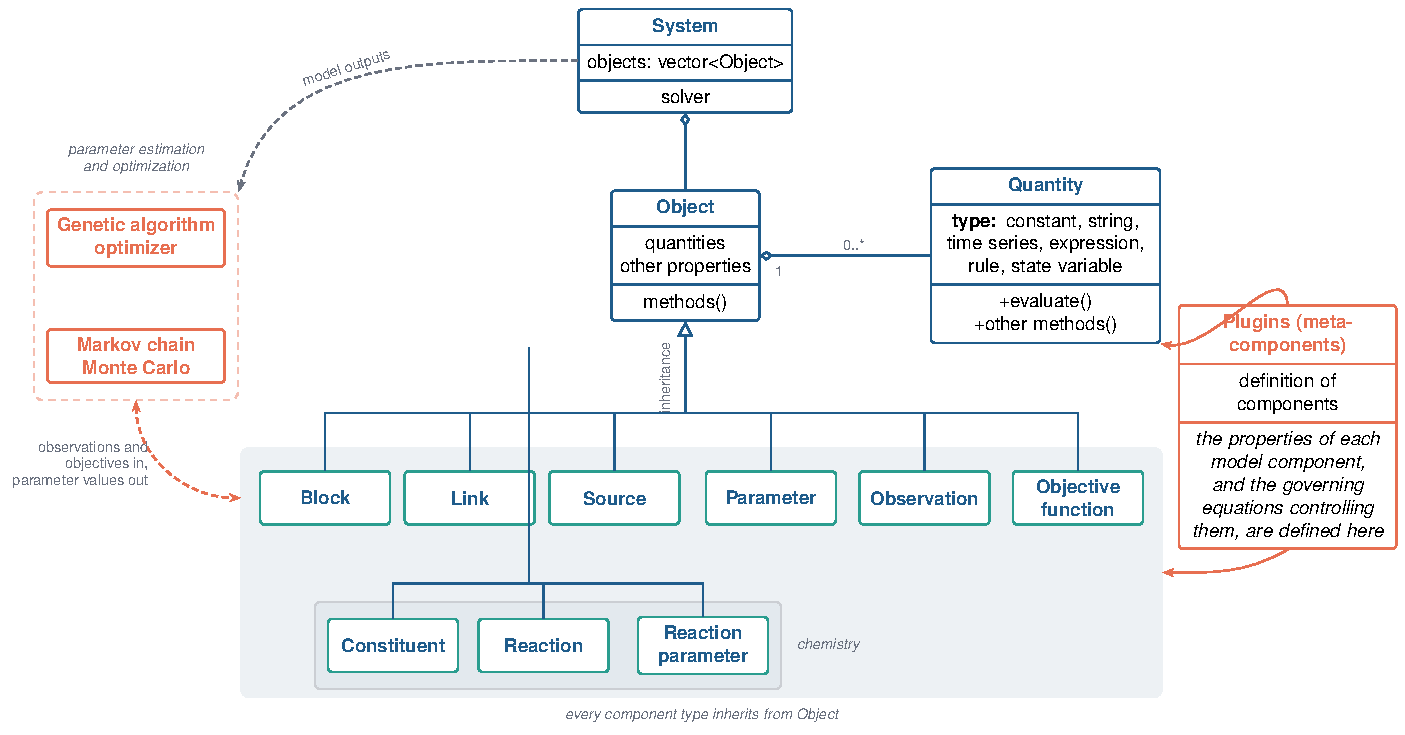
\includegraphics[width=\textwidth, height=0.80\textheight, keepaspectratio]
    {N8_framework.pdf}\par
  \vspace{0.25em}
  {\tiny\color{ohqgrey} After Fig.~1 of Massoudieh (2023),
  \emph{Environmental Modelling and Software} \textbf{164}, 105707.}
\end{frame}

\begin{frame}[fragile]{Everything is a plugin}
  \begin{columns}[T,onlytextwidth]
    \begin{column}{0.53\textwidth}
      {\tiny\color{ohqgrey}\ttfamily resources/Reservoir\_operation.json}
      \vspace{-1pt}
\begin{lstlisting}[style=ohqjsonstyle]
"Spillway": {
  "type": "link",
  "typecategory": "Connectors",
  "description": "Reservoir spillway",
  "icon": { "filename": "Splillway.png" },
  "reservoir_power": {
    "type": "value",  "default": "2",
    "description": "Reservoir rating curve power",
    "ask_user": "true", "delegate": "ValueBox",
    "estimate": "true"
  },
  "reservoir_coeff": {
    "type": "value",  "default": "10",
    "description": "Reservoir rating curve coefficient",
    "ask_user": "true", "delegate": "ValueBox",
    "estimate": "true"
  },
  "flow": {
    "type": "expression",
    "expression": "reservoir_coeff*Storage.s^reservoir_power",
    "includeinoutput": "true",
    "applylimit": "true"
  }
}
\end{lstlisting}
    \end{column}
    \begin{column}{0.44\textwidth}
      That is a complete, working component: a spillway whose discharge follows
      a power-law rating curve.
      \begin{itemize}\setlength\itemsep{2pt}
        \item \texttt{ask\_user} puts the property in the GUI form, with
              \texttt{delegate} choosing the editor widget
        \item \texttt{estimate} exposes it to calibration and MCMC
        \item \texttt{expression} is the governing equation, written in terms
              of the other properties and the connected blocks' states
        \item \texttt{applylimit} tells the solver this flux cannot drain a
              block below empty
      \end{itemize}
      No C++ and no recompile. Drop the file in and the component appears.
    \end{column}
  \end{columns}
\end{frame}

\begin{frame}{The template library}
  \vspace{-0.3em}
  % GENERATED by make_icon_grid.py -- do not edit by hand.
% Source: resources/default_templates.list (the GUI's Add-plugin menu).

\begin{columns}[T,onlytextwidth]
  \begin{column}{0.1210\textwidth}\centering
    
\includegraphics[height=\iconsize]{icons/pond_template.png}\\[2pt]
    \parbox[t][\iconlabelht][t]{\linewidth}{\centering\tiny Pond}
  \end{column}
  \begin{column}{0.1210\textwidth}\centering
    
\includegraphics[height=\iconsize]{icons/evaporation_template.png}\\[2pt]
    \parbox[t][\iconlabelht][t]{\linewidth}{\centering\tiny Evapo-\\transpiration}
  \end{column}
  \begin{column}{0.1210\textwidth}\centering
    
\includegraphics[height=\iconsize]{icons/groundwater_template.png}\\[2pt]
    \parbox[t][\iconlabelht][t]{\linewidth}{\centering\tiny Groundwater}
  \end{column}
  \begin{column}{0.1210\textwidth}\centering
    
\includegraphics[height=\iconsize]{icons/open_channel_template.png}\\[2pt]
    \parbox[t][\iconlabelht][t]{\linewidth}{\centering\tiny Open channel}
  \end{column}
  \begin{column}{0.1210\textwidth}\centering
    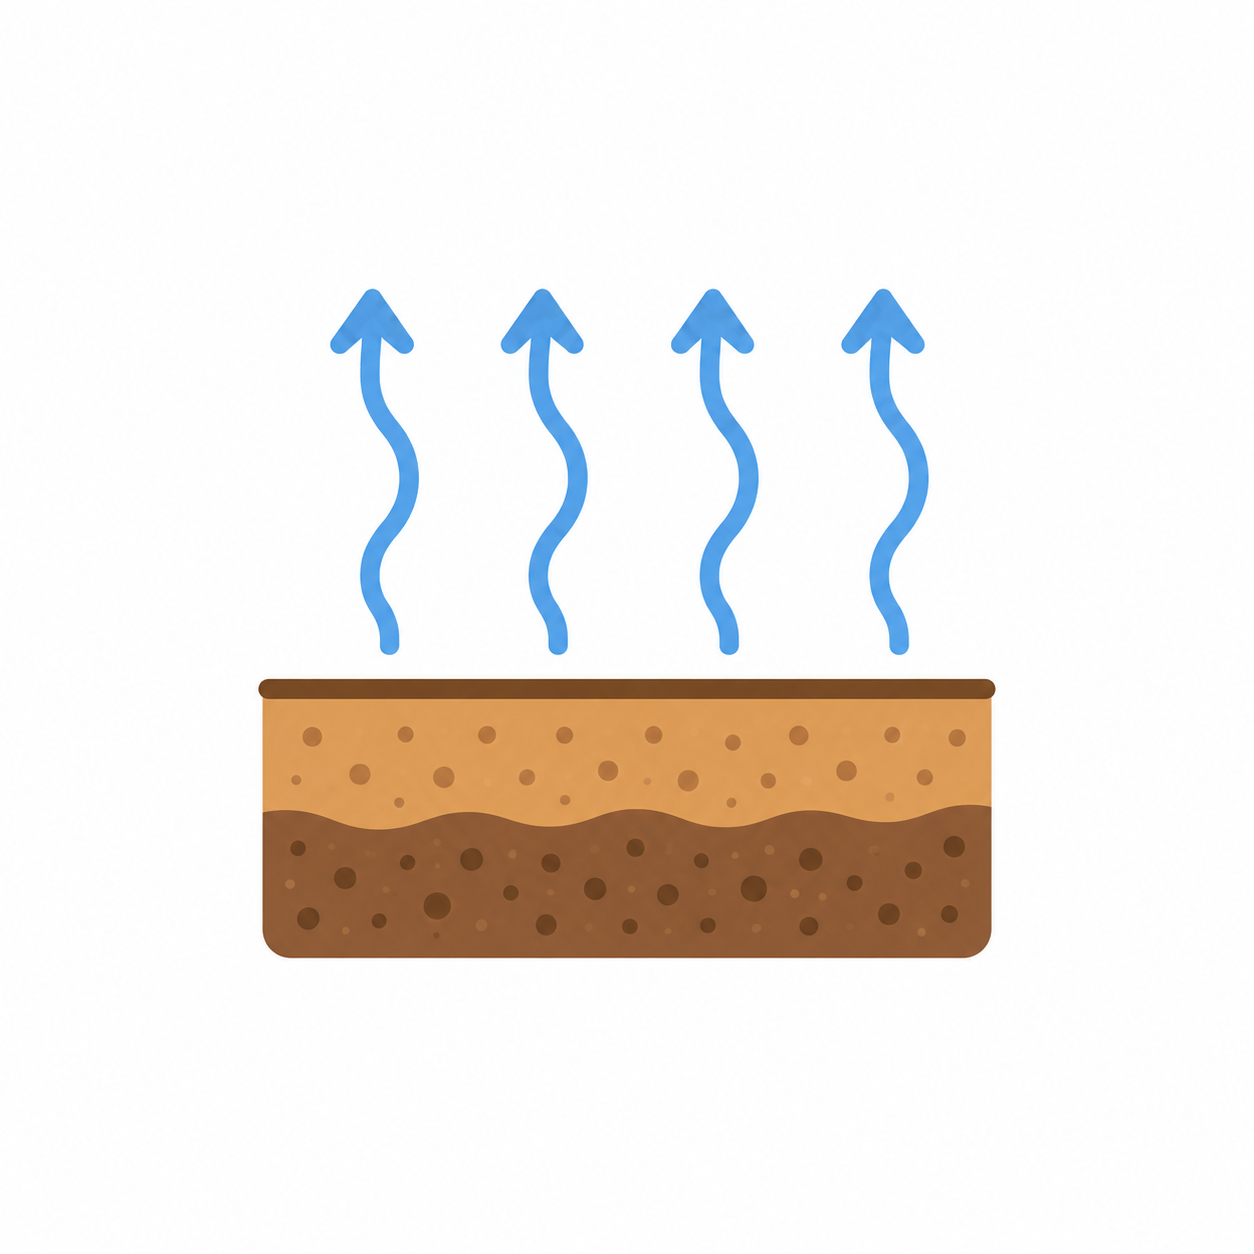
\includegraphics[height=\iconsize]{icons/soil_evaporation_template.png}\\[2pt]
    \parbox[t][\iconlabelht][t]{\linewidth}{\centering\tiny Soil evapo-\\transpiration}
  \end{column}
  \begin{column}{0.1210\textwidth}\centering
    
\includegraphics[height=\iconsize]{icons/pipe_pump_template.png}\\[2pt]
    \parbox[t][\iconlabelht][t]{\linewidth}{\centering\tiny Pipe and pump\\systems}
  \end{column}
  \begin{column}{0.1210\textwidth}\centering
    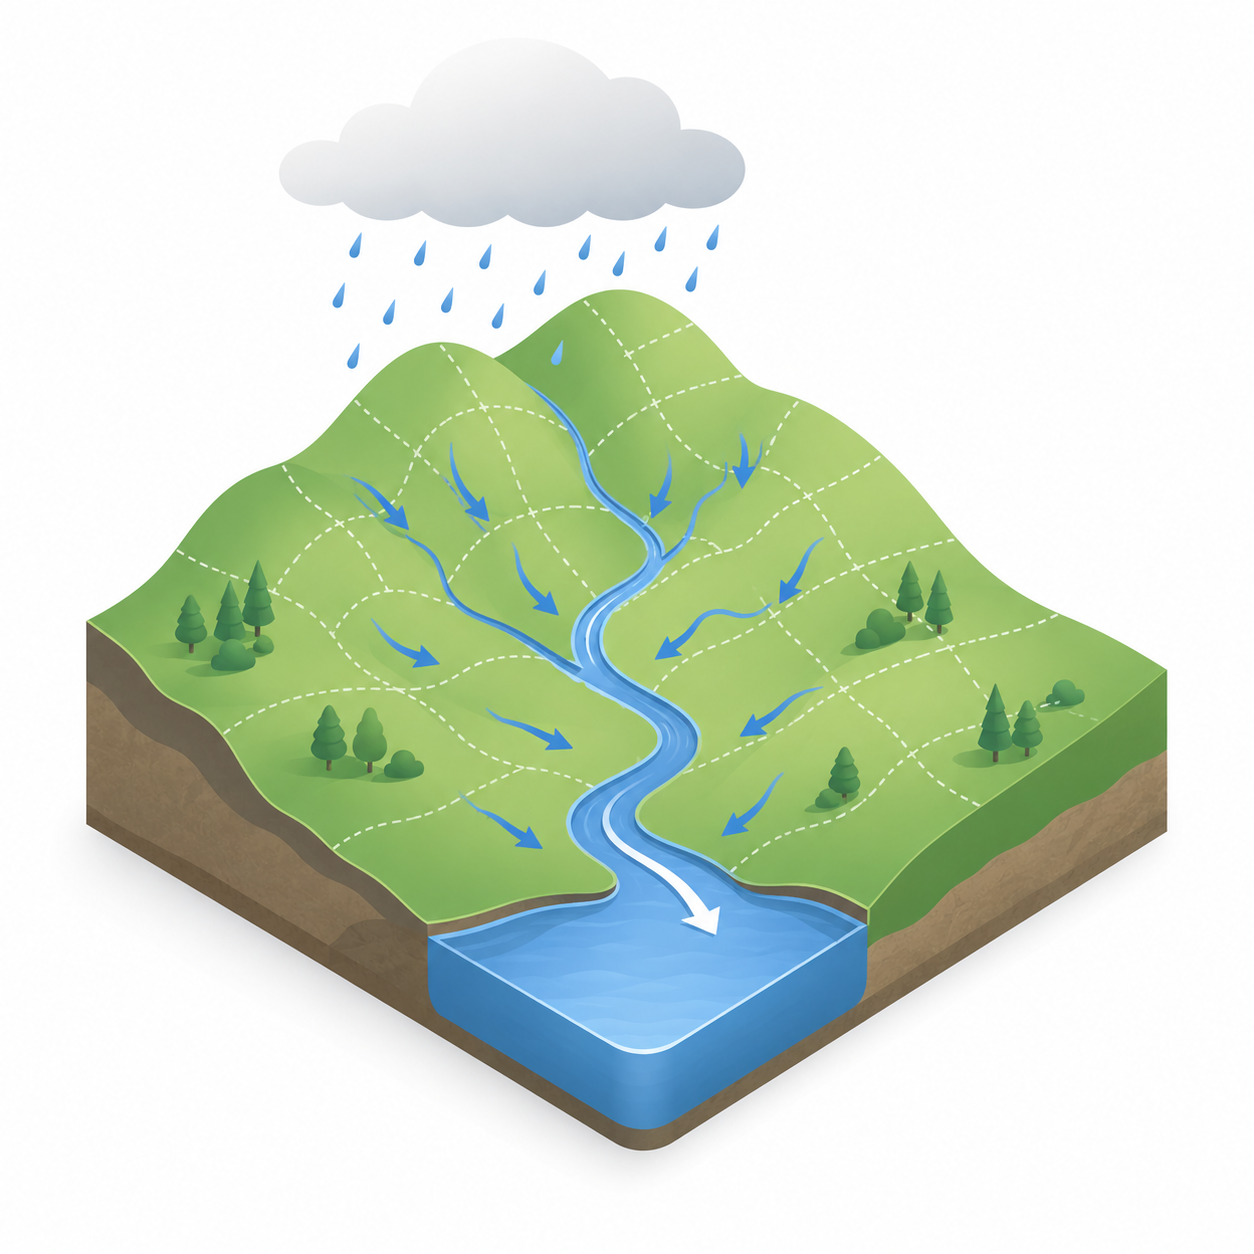
\includegraphics[height=\iconsize]{icons/rainfall_runoff_template.png}\\[2pt]
    \parbox[t][\iconlabelht][t]{\linewidth}{\centering\tiny Rainfall-runoff}
  \end{column}
  \begin{column}{0.1210\textwidth}\centering
    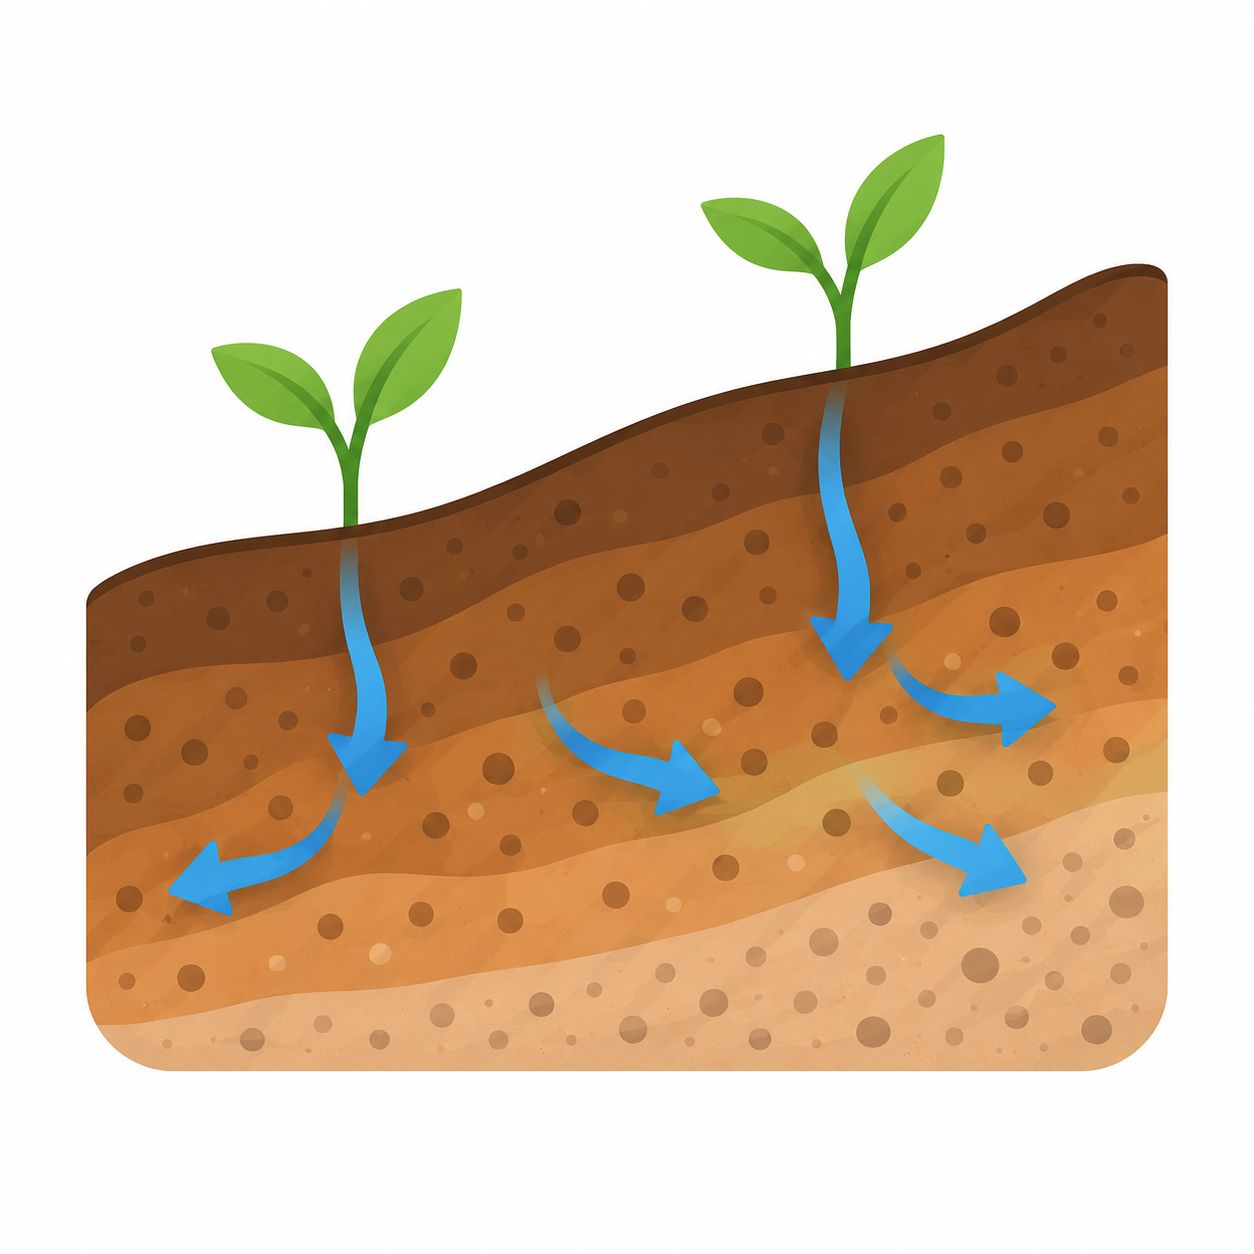
\includegraphics[height=\iconsize]{icons/soil_template.png}\\[2pt]
    \parbox[t][\iconlabelht][t]{\linewidth}{\centering\tiny Unsaturated\\soil}
  \end{column}
\end{columns}
\vspace{\iconrowgap}
\begin{columns}[T,onlytextwidth]
  \begin{column}{0.1210\textwidth}\centering
    
\includegraphics[height=\iconsize]{icons/well_template.png}\\[2pt]
    \parbox[t][\iconlabelht][t]{\linewidth}{\centering\tiny Well}
  \end{column}
  \begin{column}{0.1210\textwidth}\centering
    
\includegraphics[height=\iconsize]{icons/city.png}\\[2pt]
    \parbox[t][\iconlabelht][t]{\linewidth}{\centering\tiny Urban water\\management}
  \end{column}
  \begin{column}{0.1210\textwidth}\centering
    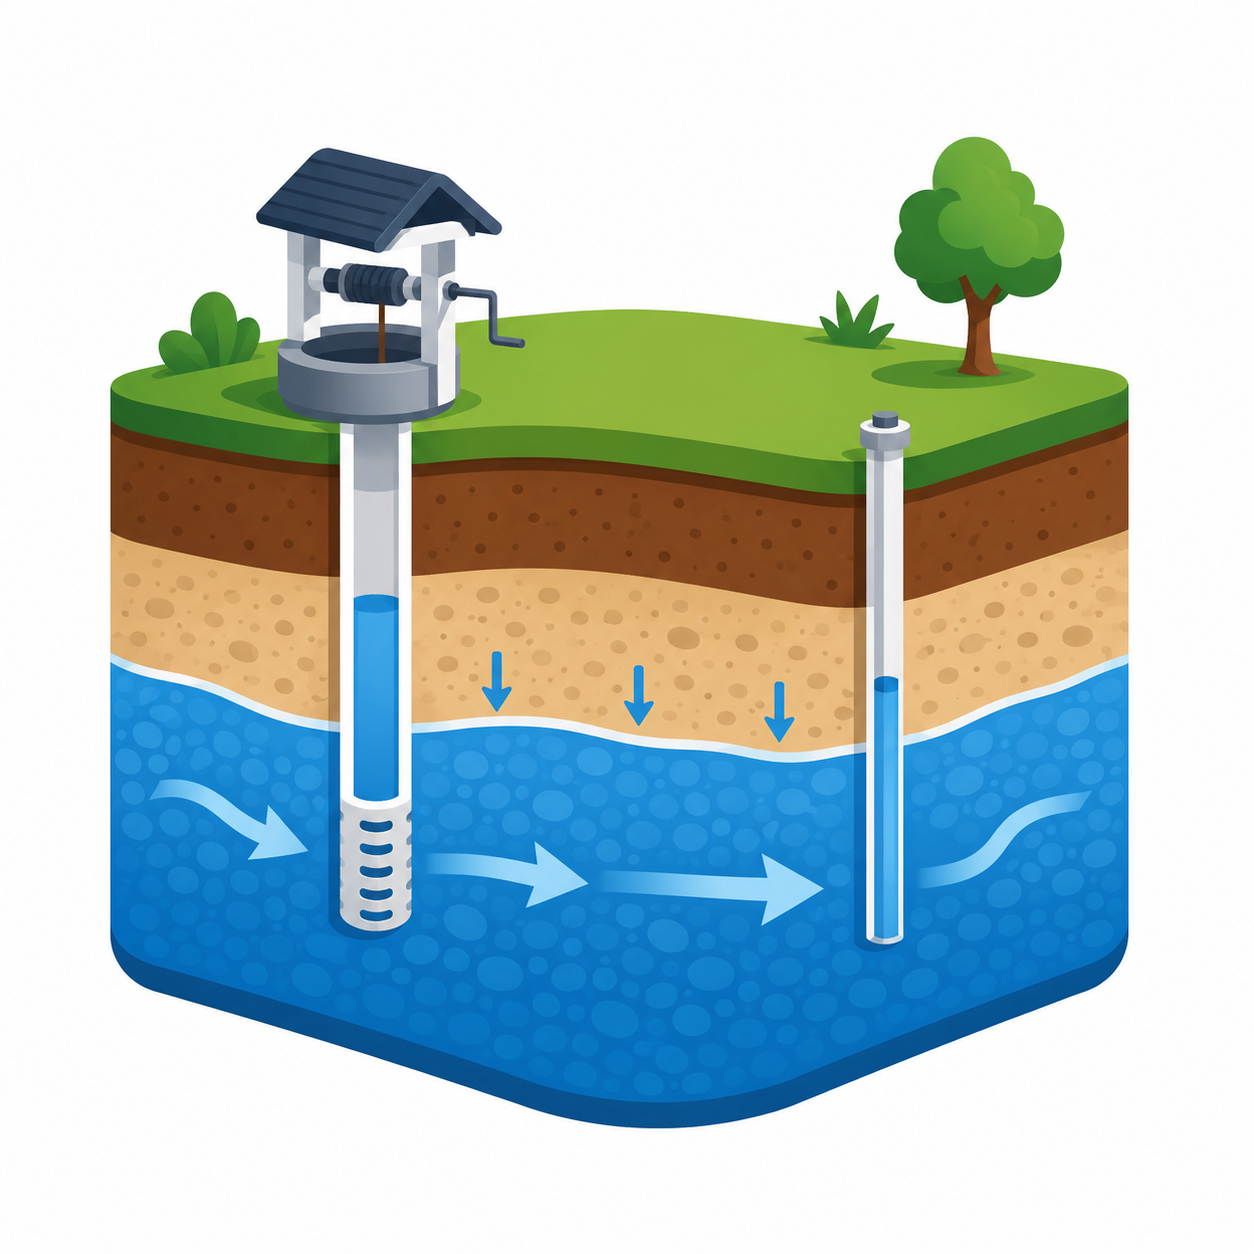
\includegraphics[height=\iconsize]{icons/unconfined_groundwater_template.png}\\[2pt]
    \parbox[t][\iconlabelht][t]{\linewidth}{\centering\tiny Unconfined\\aquifer}
  \end{column}
  \begin{column}{0.1210\textwidth}\centering
    
\includegraphics[height=\iconsize]{icons/mass_transfer_template.png}\\[2pt]
    \parbox[t][\iconlabelht][t]{\linewidth}{\centering\tiny Mass transfer}
  \end{column}
  \begin{column}{0.1210\textwidth}\centering
    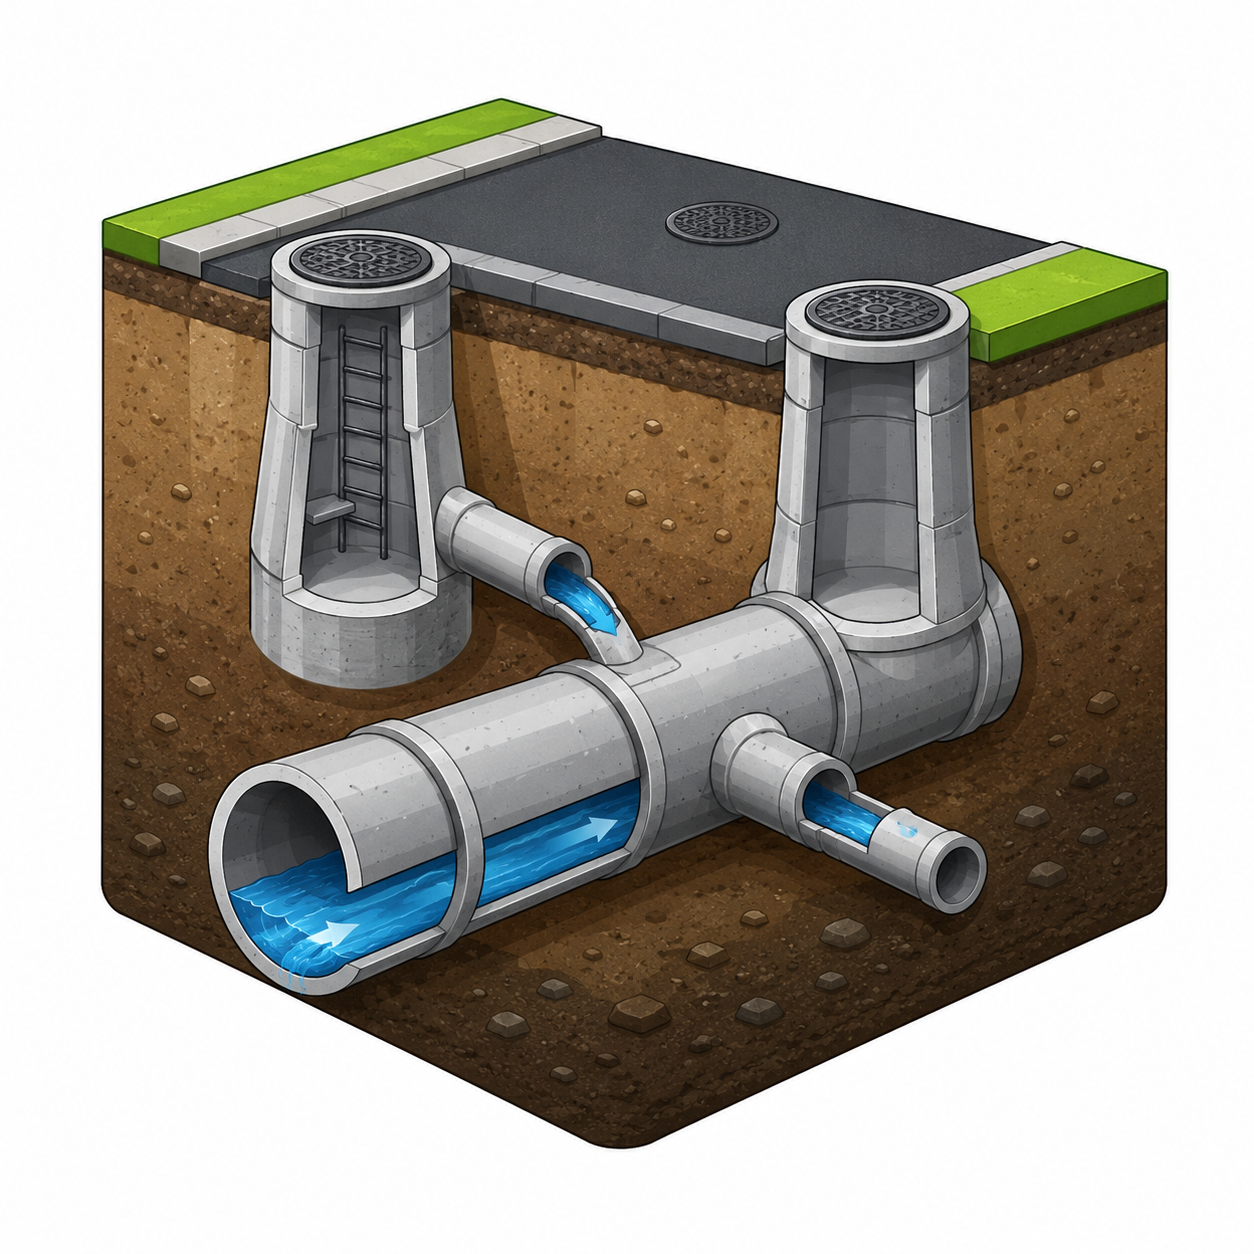
\includegraphics[height=\iconsize]{icons/Sewer_system_template.png}\\[2pt]
    \parbox[t][\iconlabelht][t]{\linewidth}{\centering\tiny Sewer system}
  \end{column}
  \begin{column}{0.1210\textwidth}\centering
    
\includegraphics[height=\iconsize]{icons/River_Template.png}\\[2pt]
    \parbox[t][\iconlabelht][t]{\linewidth}{\centering\tiny River\\processes}
  \end{column}
  \begin{column}{0.1210\textwidth}\centering
    
\includegraphics[height=\iconsize]{icons/Reservoir_template.png}\\[2pt]
    \parbox[t][\iconlabelht][t]{\linewidth}{\centering\tiny Reservoir\\operation}
  \end{column}
  \begin{column}{0.1210\textwidth}\centering
    
\includegraphics[height=\iconsize]{icons/buildup_washoff_template.png}\\[2pt]
    \parbox[t][\iconlabelht][t]{\linewidth}{\centering\tiny Build-up /\\wash-off}
  \end{column}
\end{columns}
\vspace{\iconrowgap}
\begin{columns}[T,onlytextwidth]
  \begin{column}{0.1210\textwidth}\centering
    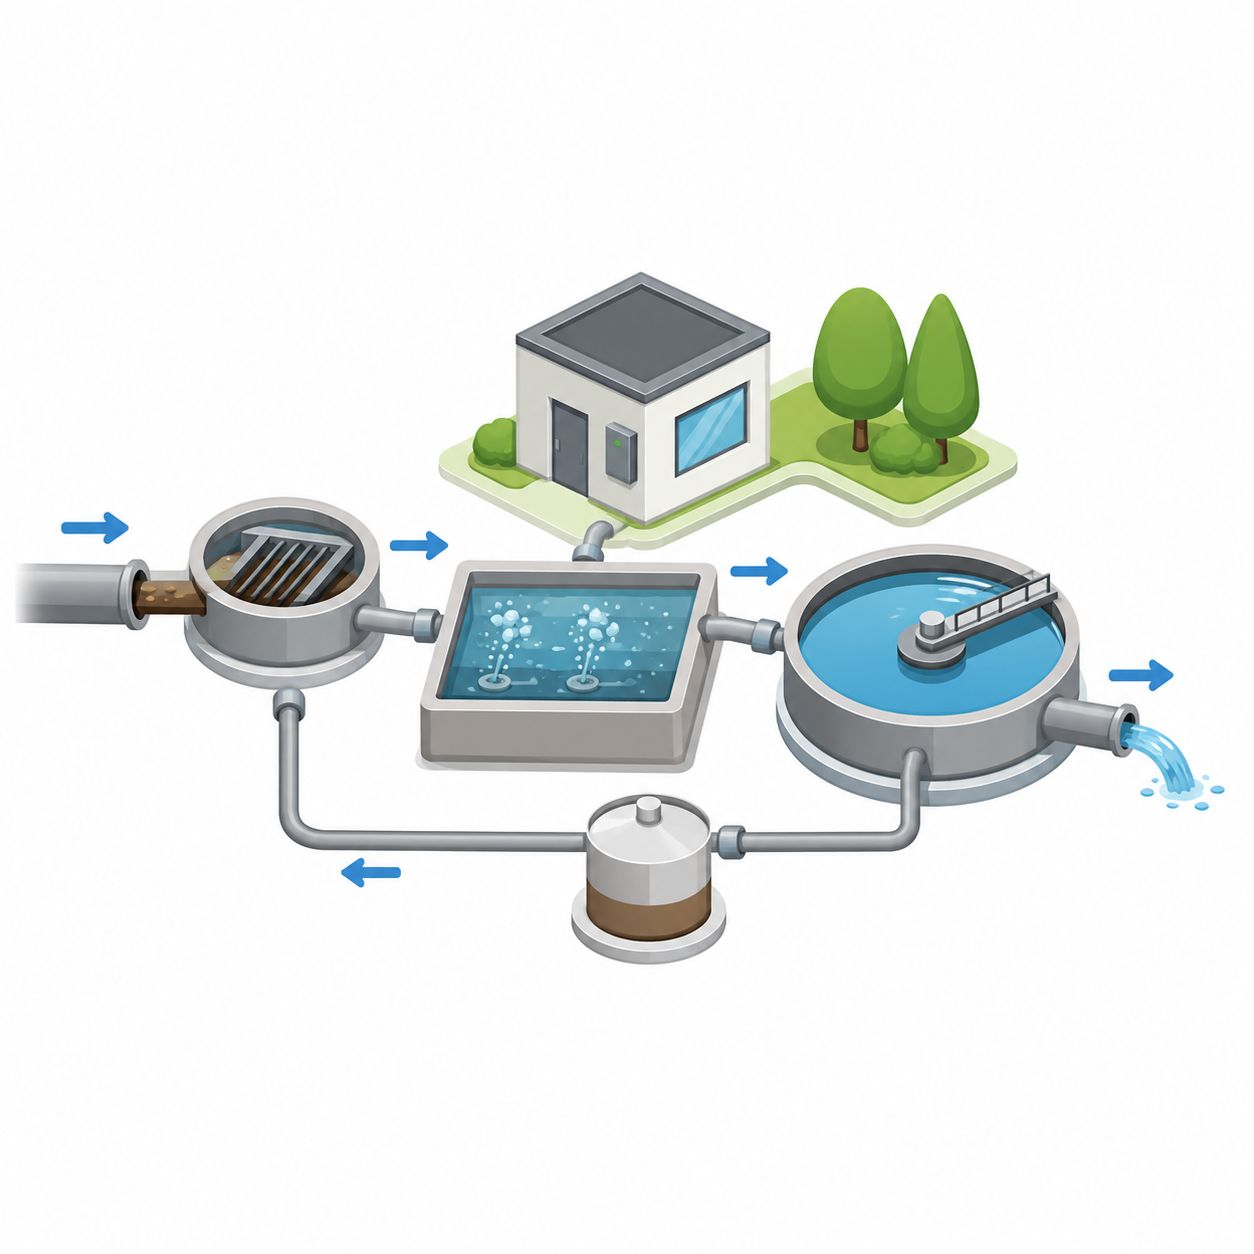
\includegraphics[height=\iconsize]{icons/wastewater_template.png}\\[2pt]
    \parbox[t][\iconlabelht][t]{\linewidth}{\centering\tiny Wastewater\\processes}
  \end{column}
  \begin{column}{0.1210\textwidth}\centering
    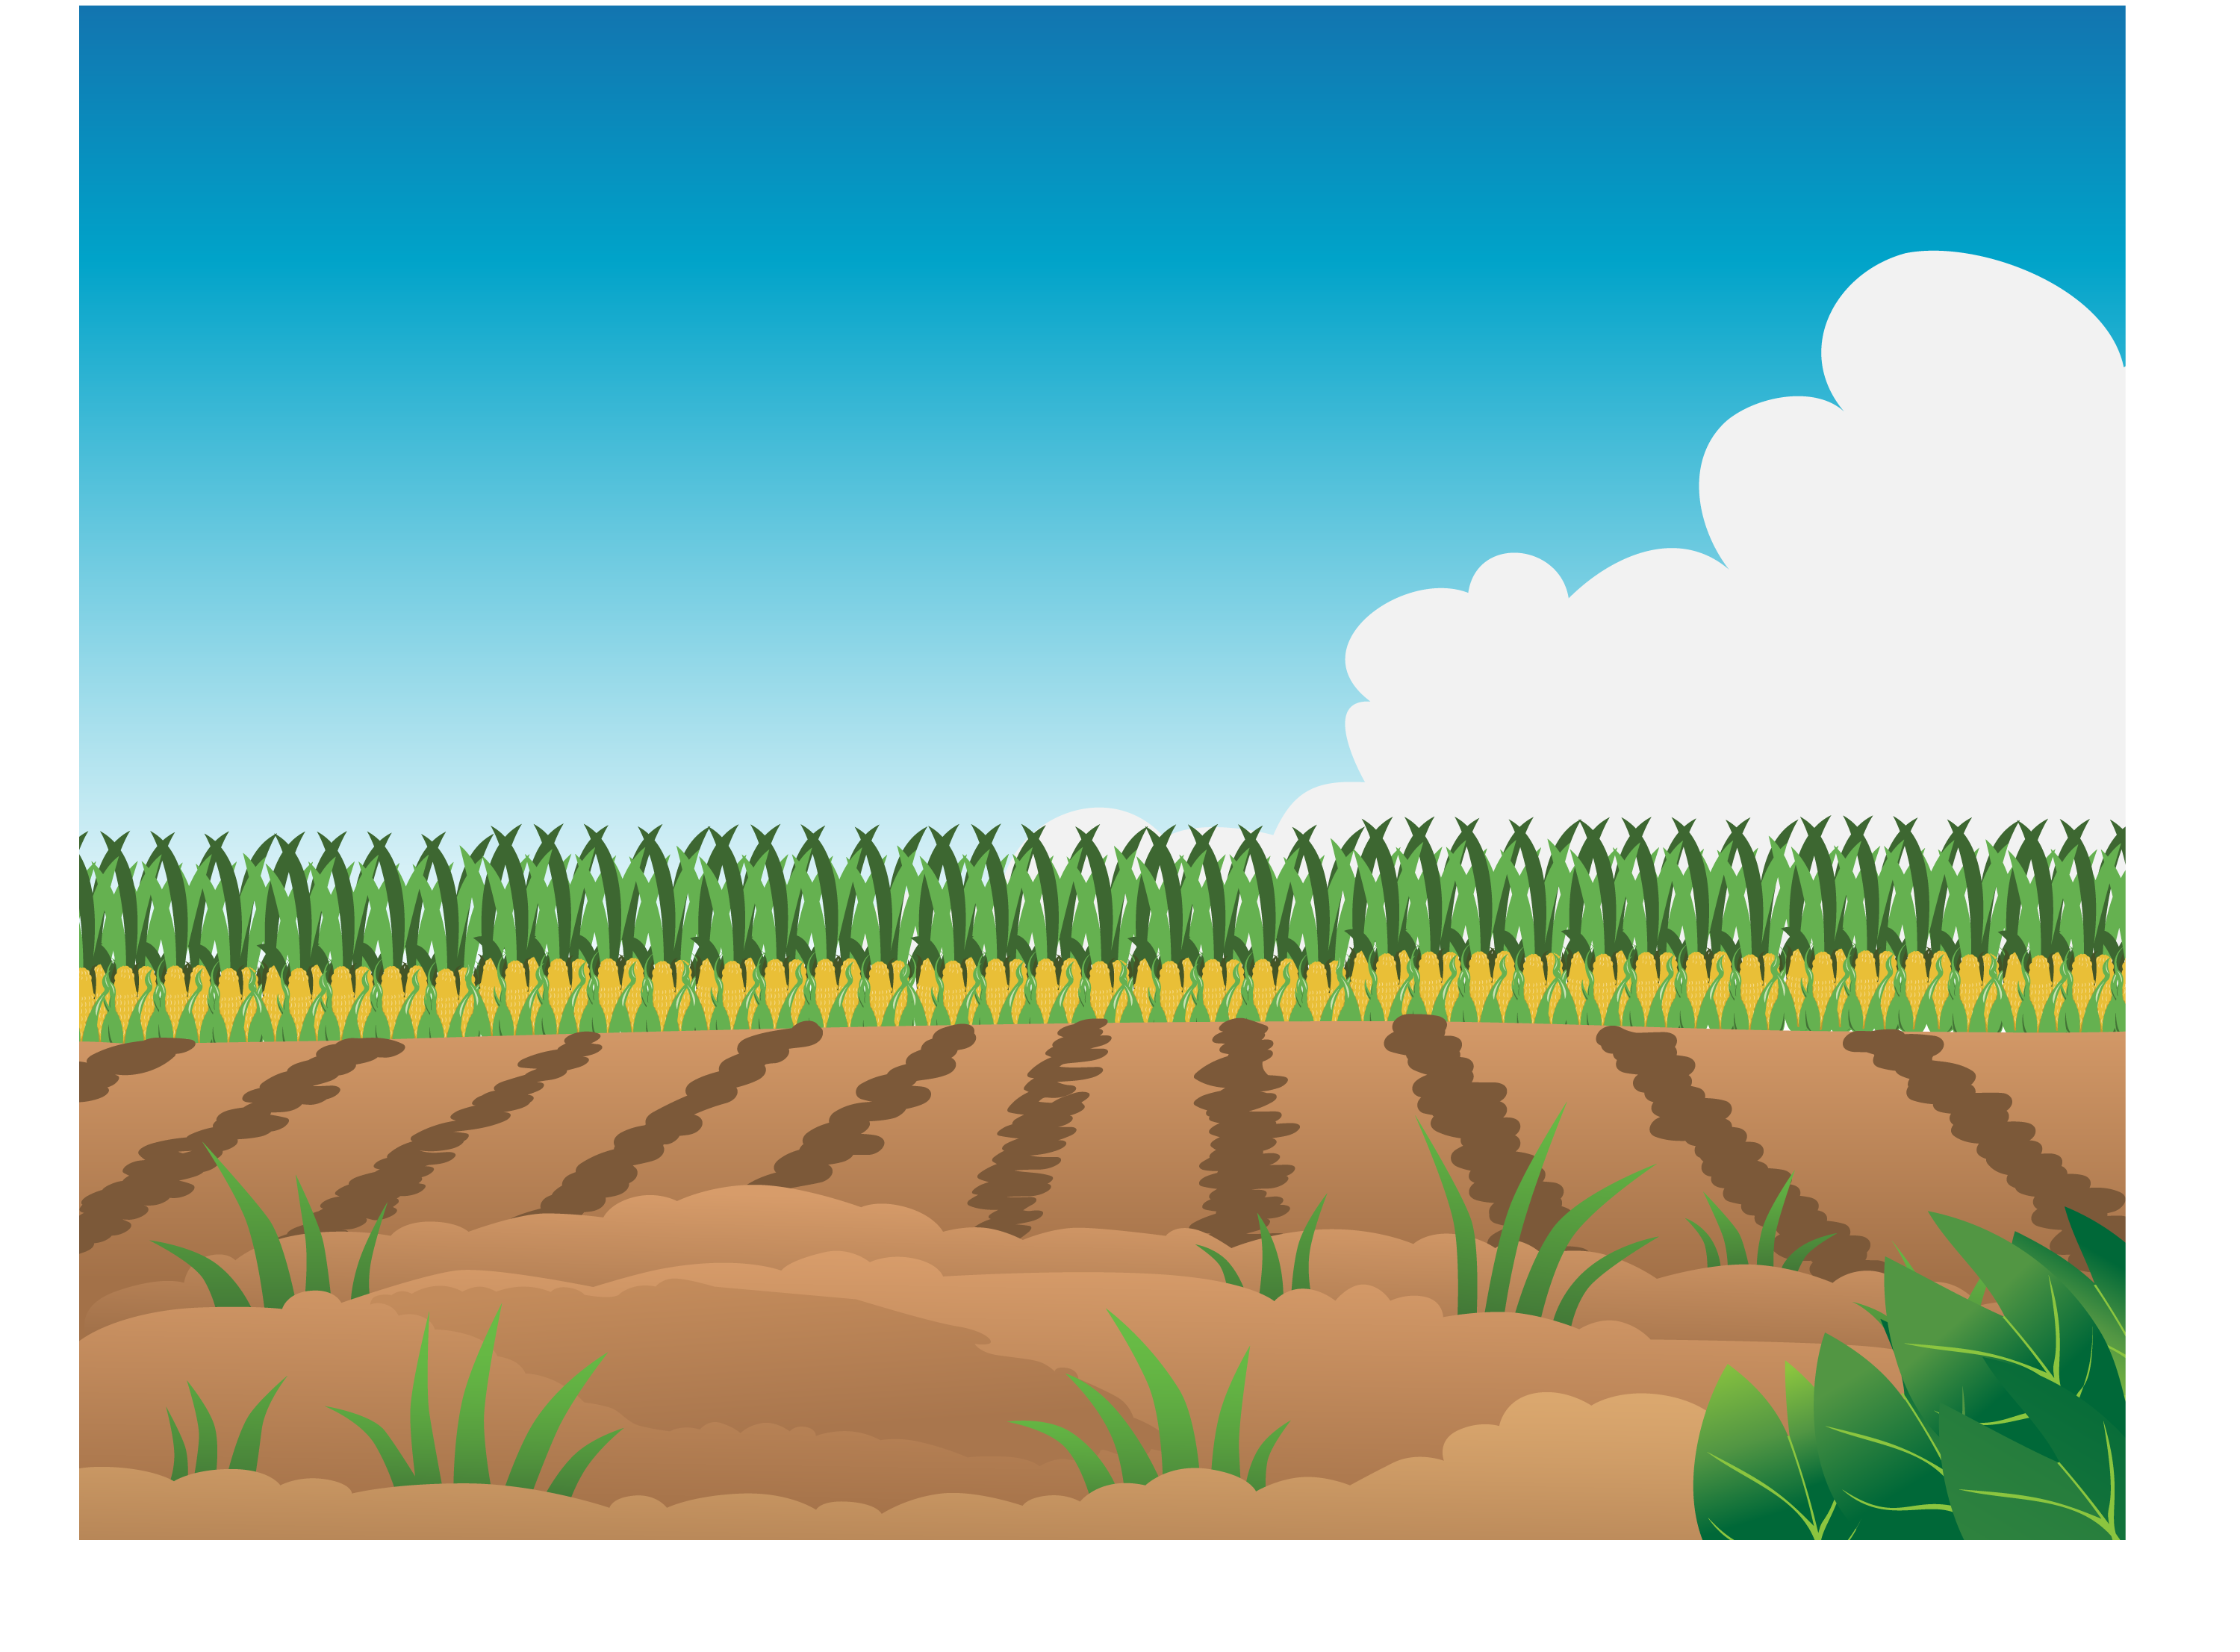
\includegraphics[height=\iconsize]{icons/plant_template.png}\\[2pt]
    \parbox[t][\iconlabelht][t]{\linewidth}{\centering\tiny Plants}
  \end{column}
  \begin{column}{0.1210\textwidth}\centering
    
\includegraphics[height=\iconsize]{icons/physicsbaseddd.png}\\[2pt]
    \parbox[t][\iconlabelht][t]{\linewidth}{\centering\tiny Physics-based\\data-driven\\hydrology}
  \end{column}
  \begin{column}{0.1210\textwidth}\centering
    
\includegraphics[height=\iconsize]{icons/hydrologic_response_unit.png}\\[2pt]
    \parbox[t][\iconlabelht][t]{\linewidth}{\centering\tiny Hydrologic\\response unit}
  \end{column}
  \begin{column}{0.1210\textwidth}\centering
    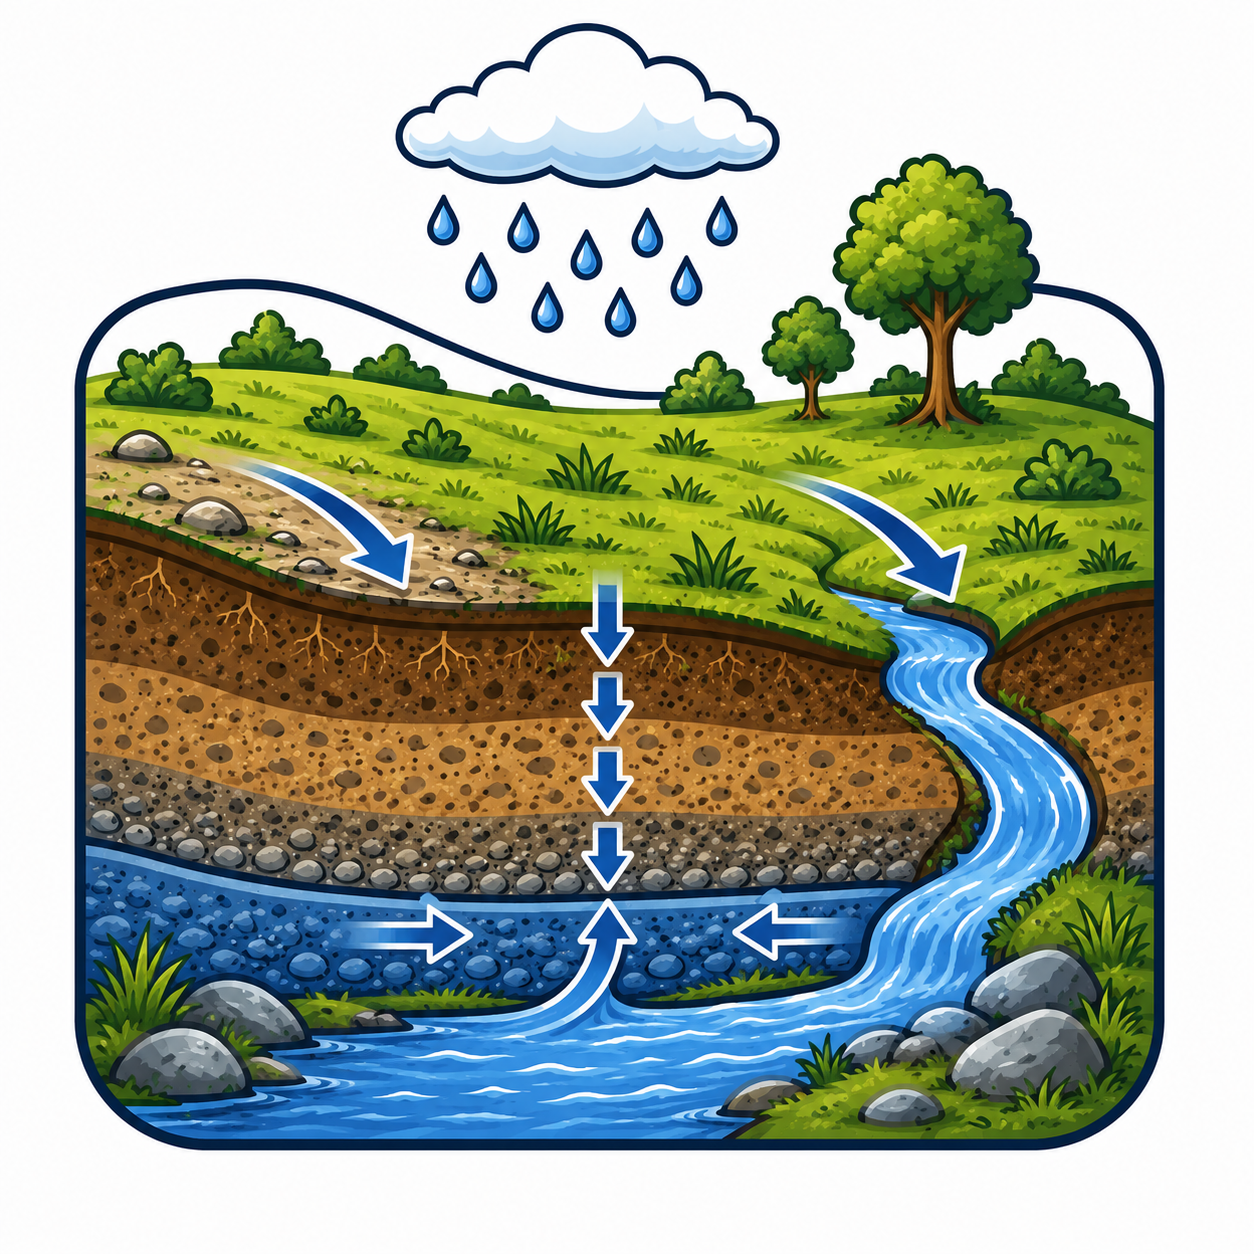
\includegraphics[height=\iconsize]{icons/mixed_hydrologic_response_unit.png}\\[2pt]
    \parbox[t][\iconlabelht][t]{\linewidth}{\centering\tiny Mixed hydrologic\\response unit}
  \end{column}
  \begin{column}{0.1210\textwidth}\centering
    
\includegraphics[height=\iconsize]{icons/cn_catchment.png}\\[2pt]
    \parbox[t][\iconlabelht][t]{\linewidth}{\centering\tiny CN catchment\\(SCS)}
  \end{column}
  \begin{column}{0.1210\textwidth}\centering
    
\includegraphics[height=\iconsize]{icons/culvert_template.png}\\[2pt]
    \parbox[t][\iconlabelht][t]{\linewidth}{\centering\tiny Culverts}
  \end{column}
  \begin{column}{0.1210\textwidth}\end{column}
\end{columns}
\vspace{\iconrowgap}

  \vspace{0.1em}
  {\scriptsize Every template above is one entry in the GUI's \alert{Add plugin}
  menu, and each is a JSON file declaring its own blocks, links, sources,
  properties and governing equations. The library grows by adding a file.}
\end{frame}

\begin{frame}[fragile]{Expressions, rules and units}
  \begin{columns}[T,onlytextwidth]
    \begin{column}{0.50\textwidth}
      {\tiny\color{ohqgrey}\ttfamily main\_components.json, Reservoir\_link\_rule}
      \vspace{-1pt}
\begin{lstlisting}[style=ohqjsonstyle]
"flow": {
  "type": "rule",
  "description": "Flow",
  "rule": {
    "Storage.s<S_min": "Q_min",
    "S_min<Storage.s<S_max":
        "Q_min+((Storage.s-S_min)/(S_max-S_min))
              *(Q_max-Q_min)",
    "Storage.s>S_max": "Q_max",
    "unit": "m^3/day;ft^3/s"
  },
  "includeinoutput": "true",
  "applylimit": "true"
}
\end{lstlisting}
      {\scriptsize A reservoir release rule: a first-match-wins chain of
      conditions, each with its own expression. Operating logic lives in the
      model, not in a script run afterwards.}
      \vspace{-2pt}
    \end{column}
    \begin{column}{0.47\textwidth}
      \begin{center}
      \figslotmini{S4}{S4_property_expressions.png}{0.58\columnwidth}{%
        Screenshot: the property box with expressions typed directly into
        property values, for instance a reaction's rate expression and its
        stoichiometric constants written in terms of other properties.}
      \end{center}
      \vspace{-2pt}
      {\scriptsize Expressions can also be typed straight into the property
      box, as in the reaction above.

      \vspace{2pt}
      Note the \texttt{unit} line on the left. \alert{Every input parameter
      carries its own unit selector}, so values go in exactly as the data
      comes, SI and US customary mixed freely in one model, converted
      internally.}
    \end{column}
  \end{columns}
\end{frame}

% =====================================================================
\section{Breadth: The Domain Sweep}
% =====================================================================

\begin{frame}{One model, several domains}
  \begin{columns}[T,onlytextwidth]
    \begin{column}{0.53\textwidth}
      The template libraries are not separate programs. Components from any of
      them go on the \alert{same canvas}, connect to each other, and are solved
      \alert{as one system of equations}.
      \vspace{0.5em}

      So a single model can carry a catchment, the sewer that drains it, the
      pumped distribution network that serves it, the pond it discharges to,
      the soil and groundwater beneath, and the water quality riding through
      all of it, with the feedbacks between them resolved at every time step
      instead of being passed between runs.
    \end{column}
    \begin{column}{0.44\textwidth}
      \textbf{\small In one network}
      \begin{itemize}\setlength\itemsep{1pt}
        \item Catchment and rainfall-runoff
        \item Sewers, gutters, catch basins
        \item Pipe networks, pumps, valves, tanks
        \item Ponds and other SCMs
        \item Unsaturated soil and groundwater
        \item Channels, culverts, reservoirs
        \item Constituents and reactions throughout
      \end{itemize}
      \vspace{0.4em}
      {\scriptsize No coupling layer, no hand-off between models, and one
      calibration over the whole system.}
    \end{column}
  \end{columns}
\end{frame}

\begin{frame}{Ready-made component libraries}
  \begin{columns}[c,onlytextwidth]
    \begin{column}{0.24\textwidth}\centering
      \gridimg{F11_Bioretention.pdf}\\{\tiny Bioretention}
    \end{column}
    \begin{column}{0.24\textwidth}\centering
      \gridimg{F11_InfiltrationBasin.pdf}\\{\tiny Infiltration basin}
    \end{column}
    \begin{column}{0.24\textwidth}\centering
      \gridimg{F11_InfiltrationTrench.pdf}\\{\tiny Infiltration trench}
    \end{column}
    \begin{column}{0.24\textwidth}\centering
      \gridimg{F11_Permeable_Pavement2.pdf}\\{\tiny Permeable pavement}
    \end{column}
  \end{columns}
  \vspace{0.8em}
  \begin{columns}[c,onlytextwidth]
    \begin{column}{0.24\textwidth}\centering
      \gridimg{F11_pond.pdf}\\{\tiny Stormwater pond}
    \end{column}
    \begin{column}{0.24\textwidth}\centering
      \gridimg{F11_Filtration.pdf}\\{\tiny Filtration}
    \end{column}
    \begin{column}{0.24\textwidth}\centering
      \gridimg{F11_ASMS.pdf}\\{\tiny Activated sludge (ASM)}
    \end{column}
    \begin{column}{0.24\textwidth}
      {\footnotesize Each of these is a \alert{parameterised template}, not a
      hard-coded model: the internal block/link structure is visible and
      editable after it is generated.}
    \end{column}
  \end{columns}
\end{frame}

% =====================================================================
\section{Depth: A Model End to End}
% =====================================================================

\begin{frame}{From schematic to running model}
  \begin{columns}[T,onlytextwidth]
    \begin{column}{0.54\textwidth}
      \fitimg[\columnwidth]{F2_bioretention_schema.png}
    \end{column}
    \begin{column}{0.42\textwidth}
      {\footnotesize
      A bioretention cell is represented by ponding storage, an engineered soil
      profile resolved as unsaturated-soil layers, an underdrain, and native-soil
      infiltration, each a block with its own state and governing equation.

      \vspace{0.5em}
      Forcing comes from precipitation and evapotranspiration sources; the
      underdrain and overflow are links with their own hydraulics.

      \vspace{0.5em}
      \alert{Nothing here is special-cased.} The same block types build a
      bioswale, a drywell, or an infiltration gallery.}
    \end{column}
  \end{columns}
\end{frame}

\begin{frame}{Model wizards: a designed BMP in a few fields}
  \begin{columns}[c,onlytextwidth]
    \begin{column}{0.40\textwidth}
      \figslotmini{S5}{S5_wizard_selection.png}{0.98\columnwidth}{%
        Screenshot: the wizard catalog.}
    \end{column}
    \begin{column}{0.58\textwidth}
      \figslotmini{S6}{S6_wizard_result.png}{0.98\columnwidth}{%
        Screenshot: the wizard's tabbed parameter form with its schematic.}
    \end{column}
  \end{columns}
  \vspace{0.3em}
  {\scriptsize Pick a control measure, then fill in design dimensions and soil
  properties on a handful of tabs, with a labelled schematic showing what each
  number means. \alert{Each field has its own unit selector}, so nothing has to
  be converted by hand on the way in. The wizard then writes a normal model:
  blocks, links, sources and all. Once generated it can be opened, inspected,
  modified and extended like anything else. No black box.}
\end{frame}

\begin{frame}[fragile]{Composite components}
  \begin{columns}[T,onlytextwidth]
    \begin{column}{0.49\textwidth}
      {\tiny\color{ohqgrey}\ttfamily resources/Composites.json}
      \vspace{-1pt}
\begin{lstlisting}[style=ohqjsonstyle]
"Bioretention_cell": {
  "type": "composite",
  "typecategory": "Composites",
  "members": {
    "Pond":      { "type": "Pond" },
    "Eng_soil":  { "type": "Soil" },
    "Aggregate": { "type": "Aggregate_storage_layer" }
  },
  "internal_links": {
    "ponding_to_soil": {
      "type": "surfacewater_to_soil_link",
      "from": "Pond", "to": "Eng_soil" },
    "soil_to_aggregate": {
      "type": "soil_to_aggregate_link",
      "from": "Eng_soil", "to": "Aggregate" }
  },
  "external_links": {
    "drain_pipe": { "from": "Aggregate", "to": "Pond" }
  }
}
\end{lstlisting}
    \end{column}
    \begin{column}{0.48\textwidth}
      A \alert{composite} groups blocks and the links between them into one
      object: one icon on the diagram and one line in the model file.
      \begin{itemize}\setlength\itemsep{2pt}
        \item The engine never sees it. Members stay ordinary blocks and links,
              so the solver, the calibration and the outputs treat them
              individually
        \item Group-level properties drive the members through mapping
              expressions, so a bioretention cell is configured once, not
              layer by layer
        \item Members are not edited separately. \alert{Ungroup} it and you are
              back to plain blocks and links, with nothing hidden
      \end{itemize}
      \vspace{0.3em}
      {\scriptsize The unit of reuse above a single block, and below a whole
      wizard-generated model.}
    \end{column}
  \end{columns}
\end{frame}

\begin{frame}{Scaling up: generated grids}
  \begin{columns}[T,onlytextwidth]
    \begin{column}{0.52\textwidth}
      \figslotmini{S7}{S7_grid_generator.png}{0.99\columnwidth}{%
        Screenshot: the Array Generator setting up a 2D soil or groundwater
        grid.}
    \end{column}
    \begin{column}{0.44\textwidth}
      \begin{itemize}\setlength\itemsep{3pt}
        \item The \alert{Array Generator} builds distributed subsurface and
              watershed models by generating block/link grids, instead of
              drawing them by hand
        \item Largest validated model to date:
              \keyfact{1{,}061 blocks / 2{,}084 links} (25\,m rainfall-driven
              watershed grid)
        \item Multi-threaded solve; sparse and dependency-graph Jacobian
              options for large systems
      \end{itemize}
    \end{column}
  \end{columns}
\end{frame}

\begin{frame}{Water quality and reactive transport}
  \begin{columns}[T,onlytextwidth]
    \begin{column}{0.52\textwidth}
      \figslotmini{S11}{S11_constituents_reactions.png}{0.95\columnwidth}{%
        Screenshot: constituent and reaction-network setup showing
        constituents, reactions, and an ASM configuration.}
    \end{column}
    \begin{column}{0.44\textwidth}
      \begin{itemize}\setlength\itemsep{3pt}
        \item \alert{Unlimited} user-defined constituents
        \item User-defined reaction networks with symbolic rate expressions
        \item Full ASM1 / ASM implementations shipped as templates
        \item Particle-size classes and sedimentation
        \item Age tracers and residence-time analysis
        \item Transport is solved on the same network as flow: one model,
              not a coupled pair
      \end{itemize}
    \end{column}
  \end{columns}
\end{frame}

\begin{frame}{Running and interpreting}
  \begin{columns}[T,onlytextwidth]
    \begin{column}{0.48\textwidth}
      \figslotmini{S8}{S8_runtime_window.png}{0.95\columnwidth}{%
        Screenshot: the runtime window during a solve, showing the progress
        bar and the adaptive time-step trace.}
    \end{column}
    \begin{column}{0.48\textwidth}
      \figslotmini{S9}{S9_results_plotter.png}{0.95\columnwidth}{%
        Screenshot: the results plotter.}
    \end{column}
  \end{columns}
  \vspace{0.3em}
  {\scriptsize While a model runs, the runtime window reports progress and
  plots what the \alert{solver} is doing: the adaptive time-step size against
  time, so a run that is struggling is visible as it happens. During
  calibration the same window plots the objective function per generation, and
  for MCMC the acceptance rate and perturbation factor per sample. Model
  results are plotted after the run, per quantity and in the unit you choose.}
\end{frame}

\begin{frame}{Learning it}
  \begin{columns}[T,onlytextwidth]
    \begin{column}{0.48\textwidth}
      \textbf{\small Knowledge base}\\[2pt]
      {\scriptsize\url{openhydroqual.com/knowledge-base}}
      \begin{itemize}\setlength\itemsep{1pt}
        \item \textbf{Theory and equations}: the full manual, writing plugins,
              composite components, CN curve method, plant plugin, culvert
              formulation
        \item \textbf{Tutorials}: foundations of blocks, links, sources and the
              mass balance; the settings reference
        \item \textbf{Examples}: pipe, pump and tank systems, open channel
              flow, reactions and transport, evapotranspiration, optimization,
              2-D unconfined aquifer flow and transport
      \end{itemize}
    \end{column}
    \begin{column}{0.48\textwidth}
      \textbf{\small YouTube channel}\\[2pt]
      {\scriptsize\url{youtube.com/@openhydroqual218}}
      \begin{itemize}\setlength\itemsep{1pt}
        \item 20 videos, including a two-part \alert{LID Conference 2026
              workshop} running about two hours
        \item Walkthroughs of the Model Wizard, including building an
              activated sludge system
        \item Worked tutorials such as oxygen sag by Streeter and Phelps in a
              plug flow reactor
      \end{itemize}
      \vspace{0.5em}
      {\scriptsize Plus a public forum on Google Groups and
      \texttt{r/OpenHydroQual} for questions.}
    \end{column}
  \end{columns}
\end{frame}

% =====================================================================
\section{The Command-Line Platform}
% =====================================================================

\begin{frame}{One model file, every entry point}
  \figslot{N3}{N3_toolchain.pdf}{0.80\textwidth}{%
    New graphic: toolchain diagram showing a single \texttt{.ohq} model file
    feeding the GUI, OHQConsole, OHQ-GA, OHQ-MCMC, the Python bindings, the
    compiled codegen kernel, and \ohtwin{}. Shows that nothing is re-entered or
    re-specified per tool. (I can draw this in TikZ.)}
\end{frame}

\begin{frame}[fragile]{Headless forward runs}
  \begin{columns}[T,onlytextwidth]
    \begin{column}{0.56\textwidth}
\begin{lstlisting}[language=bash]
$ OpenHydroQual-Console <model.ohq> [options]

  -o, --outputfile <name>  override alloutputfile
  -w, --workdir <dir>      folder for relative paths
  -r, --resources <dir>    templates (or $OHQ_RESOURCES)
  -q, --quiet              suppress per-step output
      --skip-verify        skip the criteria check

Exit codes: 0 ok, 2 usage, 3 input not found,
            4 model errors, 5 solve failed.
\end{lstlisting}
    \end{column}
    \begin{column}{0.42\textwidth}
      \begin{itemize}\setlength\itemsep{2pt}
        \item No Qt Widgets and no display, so it runs on a cluster or in CI
        \item Same solver code path as the GUI, so results are identical
        \item \alert{Distinct exit codes}, so a script can tell a converged run
              from a model that silently loaded no inflow
        \item Criteria are checked before the solve, not discovered halfway
              through it
      \end{itemize}
      \vspace{0.4em}
      {\scriptsize This is what makes \ohq{} embeddable, not only interactive:
      drive it from a \alert{GIS} workflow, stand it up \alert{on a server}
      behind a web front end, wire it into an optimisation or
      machine-learning loop, or run it as the engine of a \alert{digital
      twin}.}
    \end{column}
  \end{columns}
\end{frame}

\begin{frame}[fragile]{Python and embedded use}
  \begin{columns}[T,onlytextwidth]
    \begin{column}{0.56\textwidth}
\begin{lstlisting}[language=Python]
import openhydroqual_py as ohq

system = ohq.System()
system.load_template('main_components.json')
system.add_template('unconfined_groundwater.json')

for i in range(1, n+1):
    system.create_block(name=f'cell({i}:1)',
        type='Unconfined Groundwater cell', ...)

system.solve()
\end{lstlisting}
    \end{column}
    \begin{column}{0.40\textwidth}
      \begin{itemize}\setlength\itemsep{3pt}
        \item Build, modify, solve and save models programmatically
        \item Drives scripted scenario generation and coupling to external
              workflows (GIS, ML, optimisation)
        \item Compiled models expose a plain \alert{C ABI}, so an \ohq{} model
              can be embedded in any host program
      \end{itemize}
    \end{column}
  \end{columns}
\end{frame}

\begin{frame}{Server and browser deployment}
  \begin{columns}[T,onlytextwidth]
    \begin{column}{0.56\textwidth}
      \figslotmini{S15}{S15_greeninfraiq.png}{0.99\columnwidth}{%
        Screenshot: the GreenInfraIQ model catalogue.}
    \end{column}
    \begin{column}{0.40\textwidth}
      \textbf{\small GreenInfraIQ}\\[1pt]
      {\scriptsize\url{greeninfraiq.com}}
      \vspace{0.5em}

      {\footnotesize A public deployment of the same engine. \textbf{OHQuery}
      runs the models server side and the browser drives them, so a user picks
      a system, enters design parameters and gets results with
      \alert{nothing installed}.}
      \vspace{0.6em}

      {\scriptsize Dockerised, with a WebSocket server for interactive remote
      runs. The same pattern hosts a client's own model catalogue.}
    \end{column}
  \end{columns}
\end{frame}

\begin{frame}{A design answer, and the model behind it}
  \begin{columns}[c,onlytextwidth]
    \begin{column}{0.63\textwidth}
      \figslotmini{S16}{S16_greeninfraiq_results.png}{0.99\columnwidth}{%
        Screenshot: a GreenInfraIQ run with its aggregate results and
        download links.}
    \end{column}
    \begin{column}{0.34\textwidth}
      {\footnotesize Fill in the soil and geometry tabs, hit run, and the page
      reports the numbers a designer is after:

      \vspace{0.4em}
      \alert{73.5\% volume reduction}, with the inflow, infiltration,
      evapotranspiration and outflow volumes behind it, plus every output
      series to download.}
      \vspace{0.6em}

      {\scriptsize And a \alert{Download the OpenHydroQual Model} button. The
      web tool is a front door, not a dead end: take the generated
      \texttt{.ohq} into the desktop application and keep going.}
    \end{column}
  \end{columns}
\end{frame}

% =====================================================================
\section{Inverse Modeling and Uncertainty}
% =====================================================================

\begin{frame}{Calibration is part of the model, not a wrapper}
  \figslot{N5}{N5_inverse_workflow.pdf}{0.80\textwidth}{%
    New graphic: inverse-modelling workflow in which observations and priors feed a GA
    for a point estimate, then MCMC for the full posterior, then forward
    propagation to predictive intervals. (I can draw this in TikZ.)}

  \vspace{-0.4em}
  {\footnotesize Declaring a quantity as a \texttt{parameter} with a prior and a
  time series as an \texttt{observation} is all that is required. The same
  declaration drives the GUI's \emph{Optimize} and \emph{Inverse Run}, the
  headless runners, and the digital twin.}
\end{frame}

\begin{frame}{Genetic-algorithm calibration}
  \begin{columns}[T,onlytextwidth]
    \begin{column}{0.60\textwidth}
      \fitimg[\columnwidth]{F10_fitness_history.png}
    \end{column}
    \begin{column}{0.36\textwidth}
      \begin{itemize}\setlength\itemsep{3pt}
        \item Population-based global search, with no gradient and no
              differentiability requirement
        \item Handles the non-smooth switching behaviour real hydrologic models
              exhibit (overflow, drying, limited outflow)
        \item Multi-objective via weighted objective-function sets
        \item Restartable: \texttt{-{}-continue} re-seeds from a previous
              population
      \end{itemize}
    \end{column}
  \end{columns}
\end{frame}

\begin{frame}{Bayesian parameter estimation}
  \begin{columns}[T,onlytextwidth]
    \begin{column}{0.60\textwidth}
      \fitimg[\columnwidth]{F8_physical_parameters.png}
    \end{column}
    \begin{column}{0.36\textwidth}
      \begin{itemize}\setlength\itemsep{3pt}
        \item MCMC over the full parameter vector, with log-normal or normal
              priors per parameter
        \item Measurement-error terms ($\sigma$) estimated \alert{jointly} with
              the physical parameters
        \item Output is a posterior sample, not a single best fit, giving
              credible intervals for every parameter
        \item Realizations propagate parameter uncertainty into predictions
      \end{itemize}
    \end{column}
  \end{columns}
  \vspace{0.2em}
  {\tiny\color{ohqgrey} Note: confirm which deployment run these panels should come from.}
\end{frame}

% =====================================================================
\section{The Model Compiler}
% =====================================================================

\begin{frame}{Why compile a model?}
  \begin{columns}[T,onlytextwidth]
    \begin{column}{0.46\textwidth}
      The cost of a simulation is concentrated in residual and Jacobian
      evaluation, where the interpreter re-walks every expression tree on every
      Newton iteration.

      \vspace{0.5em}
      But a model's computational shape is \alert{static after it is loaded}.

      \vspace{0.5em}
      So \ohq{} can \alert{compile a specific model} into straight-line C++:
      no expression interpreter at run time, constants folded, quantities
      lowered to the coarsest loop level where they stay valid.
    \end{column}
    \begin{column}{0.50\textwidth}
      {\footnotesize
      Every quantity is classified by a static dependency analysis and lowered
      to the coarsest loop level where it stays valid: constants folded to
      literals, per-step quantities computed once a step, and only the
      genuinely state-dependent ones evaluated inside the Newton iteration.

      \vspace{0.6em}
      The generated folder is self-contained. It carries a header-only runtime
      and builds on a machine that has never seen OpenHydroQual, on Linux,
      macOS or Visual Studio.}
    \end{column}
  \end{columns}
\end{frame}

\begin{frame}{Measured performance}
  \centering
  \setlength{\figslotmaxht}{0.78\textheight}
  \figslot{N4}{N4_codegen_speedup.pdf}{\textwidth}{%
    New graphic: the codegen pipeline plus a speed-up bar chart against the
    interpreter, with the absolute times and the parity statistics.}
  \vspace{-0.4em}
  \parbox{\textwidth}{\scriptsize Only the \emph{solve} is replaced. Parameter
  bookkeeping, the objective function, the GA and MCMC drivers and all output
  writing are identical either way, so the two modes are
  \alert{directly comparable}.}
\end{frame}

\begin{frame}[fragile]{The pipeline and its guardrails}
\begin{lstlisting}[language=bash]
$ ohq_generate model.ohq resources/ gen_model S13 Storage --project shared
$ cmake -S gen_model -B gen_model/build -DCMAKE_BUILD_TYPE=Release
$ cmake --build gen_model/build -j
$ OHQ-MCMC model.ohq work_dir --kernel gen_model/build/libS13.so
\end{lstlisting}
  \vspace{0.3em}
  \begin{columns}[T,onlytextwidth]
    \begin{column}{0.48\textwidth}
      {\scriptsize
      The generated folder is \alert{self-contained}: a header-only runtime,
      no Qt, no Armadillo, no \ohq{} at compile time. It builds on a machine
      that has never seen the platform, on Linux, macOS or Visual Studio.}
    \end{column}
    \begin{column}{0.48\textwidth}
      {\scriptsize
      The generator \alert{refuses} to emit a kernel a calibration cannot
      drive: if an estimated parameter does not reach a settable value in the
      generated code, generation fails instead of silently ignoring it. The
      runner then re-verifies parameter and observation names against the model
      at load time.}
    \end{column}
  \end{columns}
\end{frame}

% =====================================================================
\section{OpenHydroTwin}
% =====================================================================

\begin{frame}{Why a twin}
  \begin{columns}[T,onlytextwidth]
    \begin{column}{0.47\textwidth}
      \textbf{The gap}
      \begin{itemize}\setlength\itemsep{4pt}
        \item SCMs are credited with benefits that are rarely measured
        \item Flow-grade instrumentation does not scale to a portfolio
        \item Cheap sensors give depth and moisture, not \alert{volumes}
      \end{itemize}
    \end{column}
    \begin{column}{0.47\textwidth}
      \textbf{What the twin adds}
      \begin{itemize}\setlength\itemsep{4pt}
        \item The model turns sparse readings into the quantities the credit
              is written against
        \item It keeps doing it \alert{as the asset ages}
        \item Any asset the engine can represent can be twinned
      \end{itemize}
    \end{column}
  \end{columns}
  \vspace{0.8em}
  {\tiny\color{ohqgrey} Shakouri, Kiriazes and Massoudieh (2026),
  \emph{OpenHydroTwin: a generic digital twin framework for stormwater
  infrastructure}.}
\end{frame}

\begin{frame}{How it runs}
  \begin{columns}[T,onlytextwidth]
    \begin{column}{0.58\textwidth}
      \fitimg[\columnwidth]{F4_twin_architecture.pdf}
    \end{column}
    \begin{column}{0.38\textwidth}
      \begin{itemize}\setlength\itemsep{6pt}
        \item A \alert{fast loop} runs the model on live weather and publishes
              a nowcast and a forecast
        \item A \alert{slow loop} refits the physical parameters to recent
              sensor data
        \item They meet only on the parameters, through snapshots on disk
      \end{itemize}
    \end{column}
  \end{columns}
\end{frame}

\begin{frame}{The assimilation cycle}
  \fitimgs[0.78\textwidth]{F5_assimilation_cycle.pdf}
  \vspace{0.3em}
  {\footnotesize Recent observations weigh more than old ones, so the fit
  \alert{follows the asset as it changes}. Sensor error is estimated alongside
  the physical parameters. The cycle can carry a full posterior forward by
  \alert{streaming MCMC}, not just a best estimate.}
\end{frame}

\begin{frame}{The number the credit is written against}
  \centering
  \setlength{\figslotmaxht}{0.66\textheight}
  \figslot{N9}{N9_cumulative_volume.pdf}{\textwidth}{%
    New graphic: cumulative underdrain volume, truth against the live twin.}
  \vspace{-0.3em}
  \parbox{\textwidth}{\scriptsize Two years of operation, including the
  clogging. The asset is instrumented only for depth, moisture and underdrain
  flow; the twin converts those into the \alert{cumulative volume} that
  performance accounting actually needs, and stays within \alert{0.7\%} of
  truth over the whole record.}
\end{frame}

\begin{frame}{Tracking a real system}
  \centering
  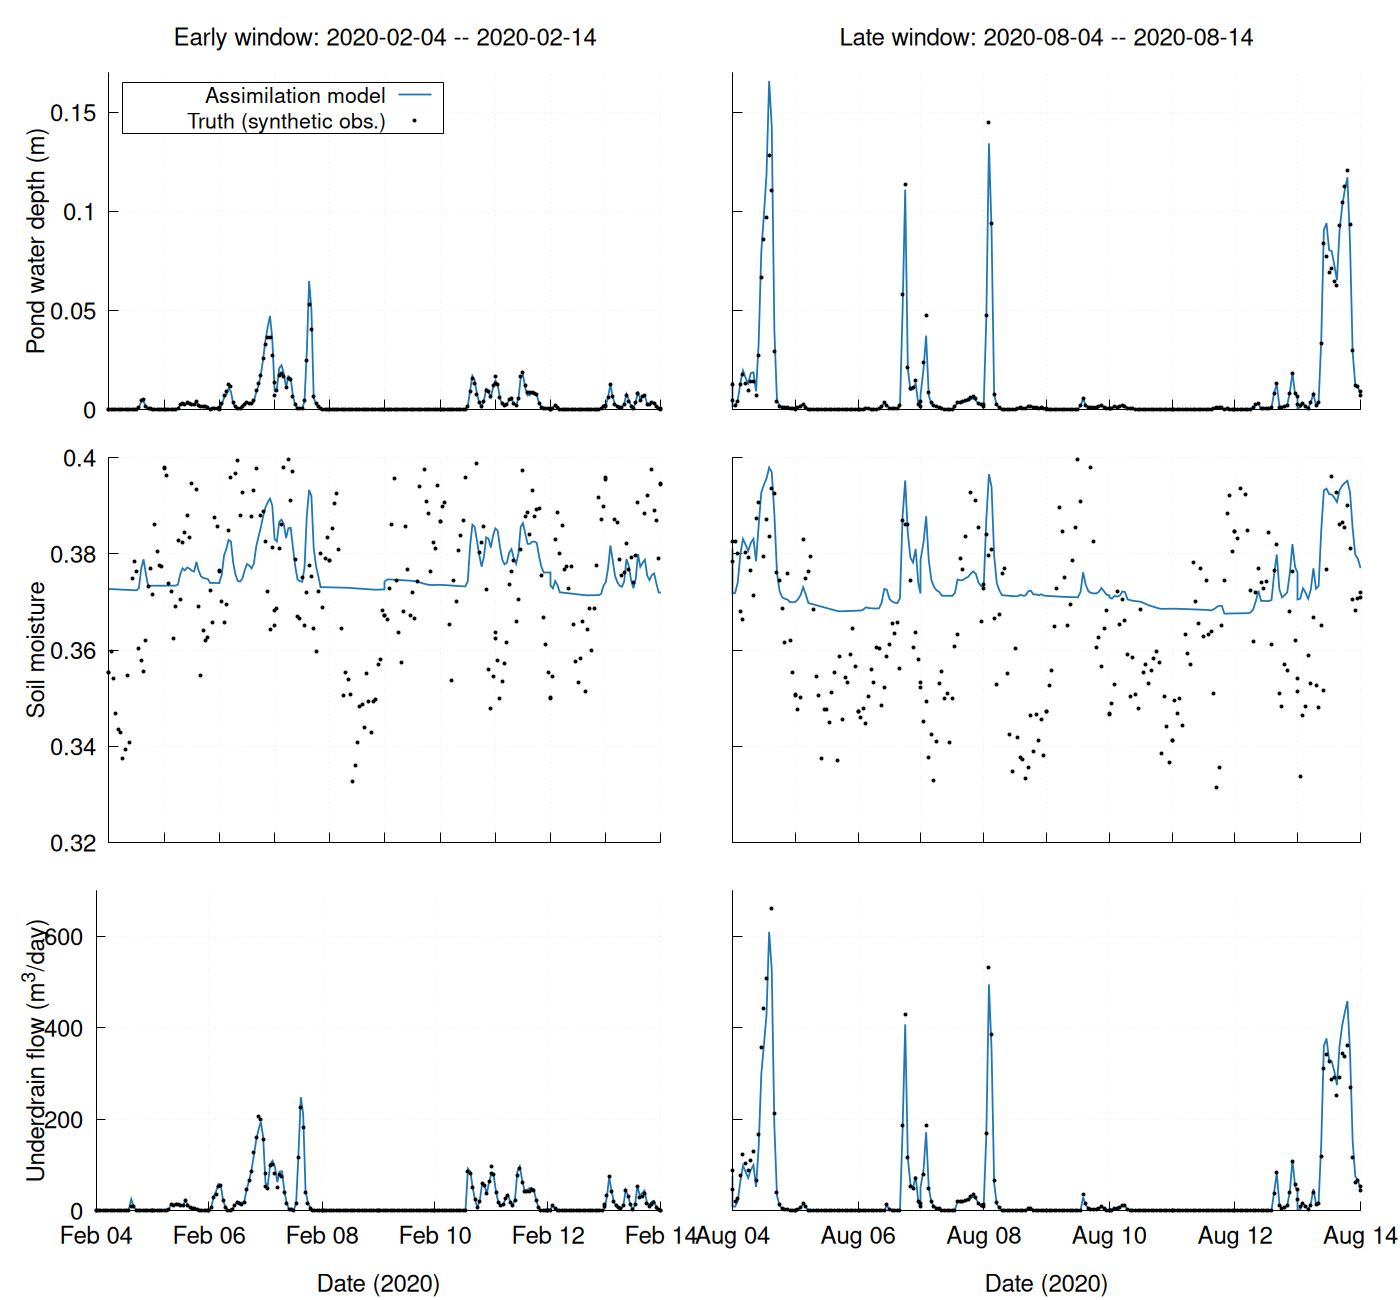
\includegraphics[width=\textwidth, height=0.80\textheight, keepaspectratio]
    {F6_truth_vs_assim.png}\par
  \vspace{0.1em}
  {\scriptsize Pond depth, soil moisture and underdrain discharge, early in the
  record and once converged.}
\end{frame}

\begin{frame}{Down to the individual storm}
  \begin{columns}[c,onlytextwidth]
    \begin{column}{0.64\textwidth}
      \figslotmini{N10}{N10_event_zoom.pdf}{0.99\columnwidth}{%
        New graphic: one storm, rain over underdrain flow and pond depth,
        truth against the twin.}
    \end{column}
    \begin{column}{0.33\textwidth}
      {\footnotesize Not just a seasonal total. The twin reproduces the
      \alert{individual event}: the peak, the recession and the secondary
      pulse a day later.

      \vspace{0.6em}
      That is the resolution operating decisions need.}
    \end{column}
  \end{columns}
\end{frame}

\begin{frame}{Parameters as a condition signal}
  \begin{columns}[c,onlytextwidth]
    \begin{column}{0.66\textwidth}
      \figslotmini{N6}{N6_drift_detection.pdf}{0.99\columnwidth}{%
        Real output of the drift run: estimated conductivity with its credible
        band, against the imposed clogging.}
    \end{column}
    \begin{column}{0.31\textwidth}
      {\footnotesize Media clogs. Conductivity falls.

      \vspace{0.6em}
      The twin refits continuously, so the \alert{parameter trajectory itself}
      reports asset condition, with an uncertainty band around it.

      \vspace{0.6em}
      Here the imposed drop from 10 to 2\,m/day is recovered, and a
      change-detection test on the same trajectory raises an alarm while the
      estimate is still moving.}
    \end{column}
  \end{columns}
\end{frame}

\begin{frame}{What the operator sees}
  \centering
  \setlength{\figslotmaxht}{0.74\textheight}
  \figslot{S14}{S14_twin_viewer.png}{\textwidth}{%
    Screenshot: the \ohtwin{} browser viewer on a live deployment.}
  \vspace{-0.4em}
  \parbox{\textwidth}{\scriptsize A browser, nothing installed. The schematic
  carries \alert{live state}: moisture in each soil layer, pond and catch-basin
  storage, and the flux on every arrow. \alert{Current} and \alert{Forecast}
  switch between where the asset is now and where it is heading.}
\end{frame}

% =====================================================================
\section{Practicalities}
% =====================================================================

\begin{frame}{Licensing, support and community}
  \begin{columns}[T,onlytextwidth]
    \begin{column}{0.48\textwidth}
      \textbf{Licensing}
      \begin{itemize}\setlength\itemsep{2pt}
        \item \alert{GNU AGPLv3} for academic and research use, free and
              source available
        \item Separate \alert{commercial license} for use in proprietary
              software or commercial products
        \item Model files, plugins and generated code are yours
      \end{itemize}
      \vspace{0.6em}
      \textbf{Platforms}
      \begin{itemize}\setlength\itemsep{2pt}
        \item Windows, macOS, Linux (AppImage, \texttt{.deb}, installer)
        \item Docker image for server deployment
      \end{itemize}
    \end{column}
    \begin{column}{0.48\textwidth}
      \textbf{Documentation}
      \begin{itemize}\setlength\itemsep{2pt}
        \item Knowledge base: theory and equations, tutorials, worked examples
        \item \url{openhydroqual.com/knowledge-base}
        \item \url{youtube.com/@openhydroqual218}
      \end{itemize}
      \vspace{0.6em}
      \textbf{Community}
      \begin{itemize}\setlength\itemsep{2pt}
        \item Public forum (Google Groups)
        \item \texttt{r/OpenHydroQual}
        \item \url{www.OpenHydroQual.com}
      \end{itemize}
    \end{column}
  \end{columns}
\end{frame}

\begin{frame}{Where this is going}
  \figslot{N7}{N7_roadmap.pdf}{0.72\textwidth}{%
    New graphic: roadmap timeline covering real-time control and optimisation,
    machine-learning integration, web-based model setup and visualisation,
    auto-generated plugin documentation, analytical Jacobian in codegen.
    (I can draw this in TikZ.)}
\end{frame}

\begin{frame}[standout]
  Questions
  \vspace{0.8em}

  {\normalsize
  Arash Massoudieh\\
  \texttt{massoudieh@cua.edu}\\
  \url{www.OpenHydroQual.com}}
\end{frame}

% =====================================================================
\appendix
% =====================================================================

\begin{frame}[allowframebreaks]{Figure checklist \hfill {\small\normalfont\figurestats}}
  {\footnotesize Each item below is an empty \texttt{\textbackslash figslot}.
  Drop the file into \texttt{figures/} under the exact name shown and rebuild.
  No edits to the source are needed. (14 figures already supplied from the
  \ohq{} and \ohtwin{} repositories are in place and not listed here.)}
  \vspace{0.4em}
  \printfigurechecklist
\end{frame}

\end{document}
